\documentclass[../../main.tex]{subfiles}

\begin{figure}[h]
    \centering
    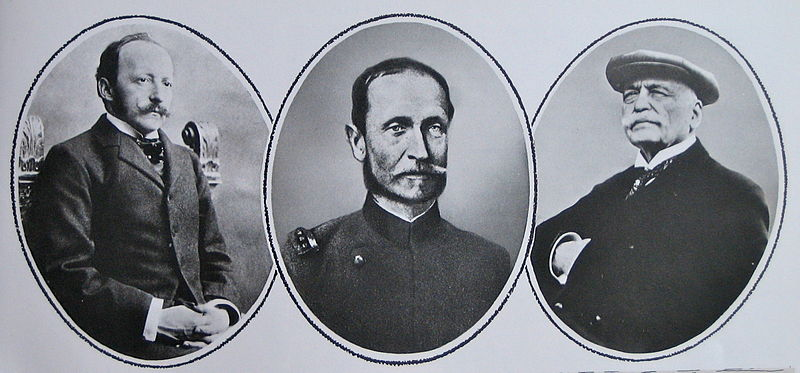
\includegraphics[width=\textwidth]{images/pfyffer.jpg}
    \caption[{Max Alphons Pfyffer (o.J.). Wikipedia. (02. Januar 2010). \newline URL: https://commons.wikimedia.org/wiki/File:C\%C3\%A9sar\_Ritz,\_Max\_Pfyffer,\_Auguste\_Escoffier.jpg [Stand 22.08.2019] }] {Max Alphons Pfyffer (in der Mitte)}
\end{figure}

Max Alphons Pfyffer wurde am 12. Oktober 1834 in Altishofen geboren und wuchs im Adel auf. Er war der Sohn von Heinrich Pfyffer von Altishofen. Die Familie Pfyffer von Altishofen war die mächtigste der Patrizierfamilien in der früheren Republik Luzern, welche die wichtigen Ämter in Luzern besetzten. Luzern war damals noch eine freie und souveräne eidgenössische Stadt und Republik.

Pfyffer war Architekt und Hotelier, er erbaute das Grand Hotel National in Luzern, welches heute noch immer in Betrieb ist. Das Hotel steht unter Denkmalschutz, es wird als Kulturgut von nationaler Bedeutung eingestuft.

Pfyffer zeichnete die Pläne für die Alpenfestung Gotthard, welche auch gebaut wurde. Dadurch wurde Max Alphons Pfyffer zum Begründer des Reduit-Konzepts.

Er starb am 12. Januar 1890 55-jährig in Luzern.